\documentclass[slidestop,usenames,dvipsnames]{beamer}
\usepackage[utf8]{inputenc}
\usepackage{fancyvrb}
\usepackage[absolute,overlay]{textpos}

\title{Commit Rater}
\subtitle{Data Extraction}
\author{Marco Brack \and Carsten Hartenfels}
\date{2015-06-09}


\beamertemplatenavigationsymbolsempty
\usetheme{Boadilla}
\usecolortheme{whale}
\setbeamertemplate{itemize items}[default]
\setbeamertemplate{enumerate items}[default]
\defbeamertemplate*{footline}{my infolines theme} {
    \leavevmode
    \hbox{
    \begin{beamercolorbox}[wd=.333333\paperwidth,ht=2.25ex,dp=1ex,center]{author in head/foot}
        \usebeamerfont{author in head/foot}\insertshortauthor
    \end{beamercolorbox}
    \begin{beamercolorbox}[wd=.333333\paperwidth,ht=2.25ex,dp=1ex,center]{title in head/foot}
        \usebeamerfont{title in head/foot}\insertshorttitle
    \end{beamercolorbox}
    \begin{beamercolorbox}[wd=.309\paperwidth,ht=2.25ex,dp=1ex,center]{date in head/foot}
        \usebeamerfont{date in head/foot}\insertshortdate{}\hspace*{2em}
        \insertframenumber{} / \inserttotalframenumber\hspace*{2ex}
    \end{beamercolorbox}}
    \vskip0pt
}

\newcounter{FrameCounter}
\newcommand{\nextframe}[0]{\stepcounter{FrameCounter}}
\newcommand{\framecount}[1]{\frametitle{\arabic{FrameCounter}. {#1}}}
\newcommand{\fitem}{\pause\vfill\item}
\newcommand{\gitem}{\vfill\item}
\newcommand{\fimage}[2]{\pause\vfill\begin{center}\includegraphics[width={#2}]{#1}\end{center}}

\begin{document}

\begin{frame}
    \titlepage
    \begin{center}
        \url{https://github.com/hartenfels/Commit-Rater}
    \end{center}
\end{frame}


%%%%%%%%%%%%%%%%%%%%%%%%%%%%%%%%%%%%%%%%%%%%%%%%%


\begin{frame}
    \frametitle{Content}
    \begin{itemize}
        \gitem Research Question
        \gitem Data Source
        \gitem Showcase
        \gitem Related Work
    \end{itemize}
\end{frame}

\nextframe
\begin{frame}
    \framecount{Research Question}
    \begin{itemize}
        \fitem How to Rate Commits?
        \begin{itemize}
            \fitem Best and Worst Practices
            \fitem Formal appearance
            \fitem Empty or Useless Messages (``Fix'', ``Bug'')
            \fitem Not considered: Information Content
        \end{itemize}
    \end{itemize}
\end{frame}


\nextframe
\begin{frame}
    \framecount{Data Source}
    \begin{itemize}
        \fitem Git Repositories:
        \begin{itemize}
            \fitem 101worker (2000+ commits)
            \fitem Mozilla OpenBadges BadgeKit (720 commits)
            \fitem Our Own Repository (75+ commits)
        \end{itemize}
    \end{itemize}
\end{frame}


\nextframe
\begin{frame}
    \framecount{Dataflow}
    \begin{itemize}
        \fitem Clone From Git Into Local Repo
        \fitem Extract Commit Data and Diffs Into Raw Data
        \fitem Process Raw Data Into an Analyzable Format
    \end{itemize}
\end{frame}


\nextframe
\begin{frame}
    \framecount{Raw data}
    \begin{itemize}
        \fitem List of Authors
        \fitem Commits by Author
        \fitem Changes in Commit
    \end{itemize}
\end{frame}


\nextframe
\begin{frame}
    \framecount{Challenges}
    \begin{itemize}
        \fitem Mapping Author Meta Data to Developers
        \fitem Determine Tense of Commit Messages
        \fitem Filtering Merges
    \end{itemize}
\end{frame}


\nextframe
\begin{frame}
    \framecount{Showcase}
    \vfill
    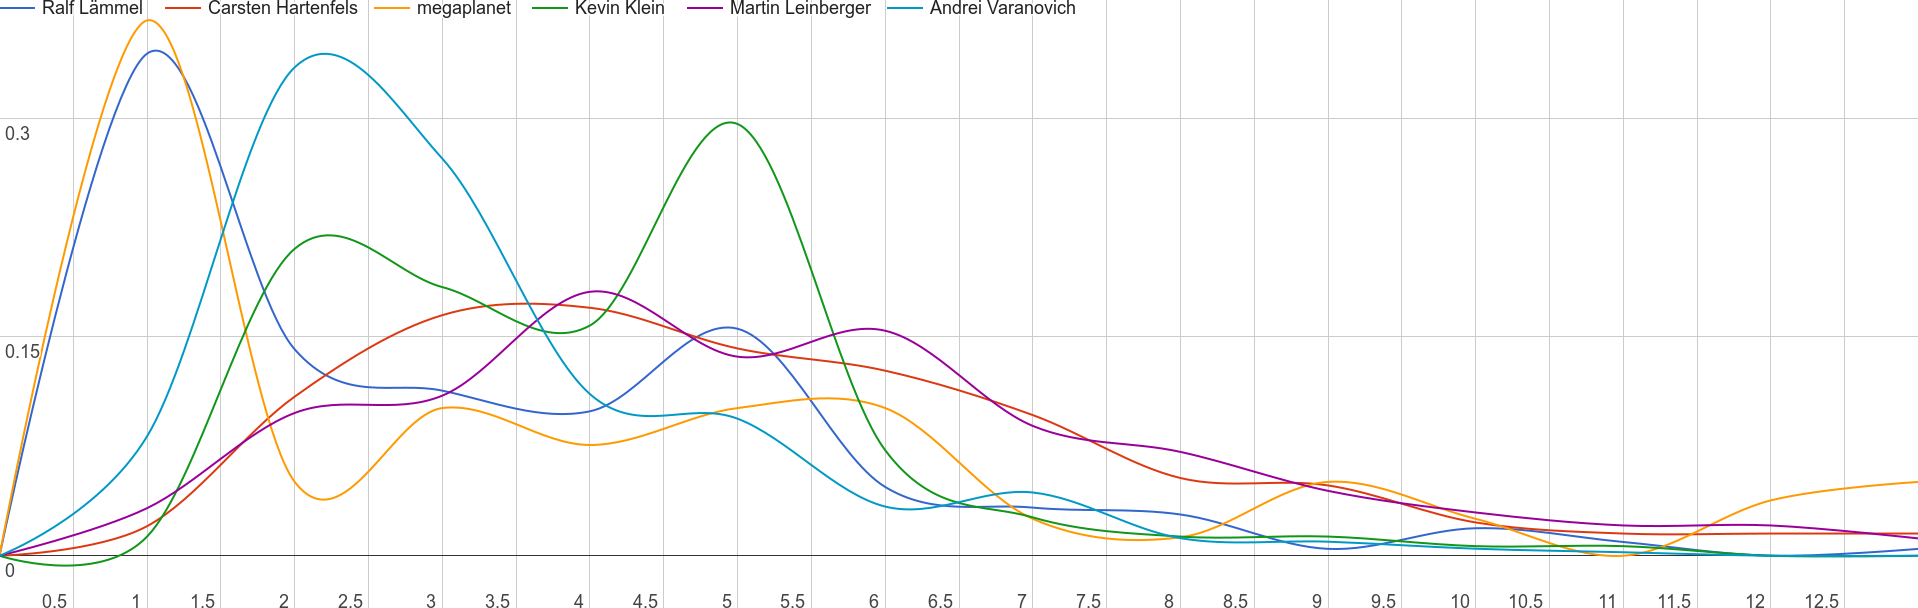
\includegraphics[width=\textwidth, clip=true, trim=0 0 700px 0]{img/101worker-wordCounts}
    \vfill
\end{frame}


\nextframe
\begin{frame}
    \framecount{Related Work}
    \pause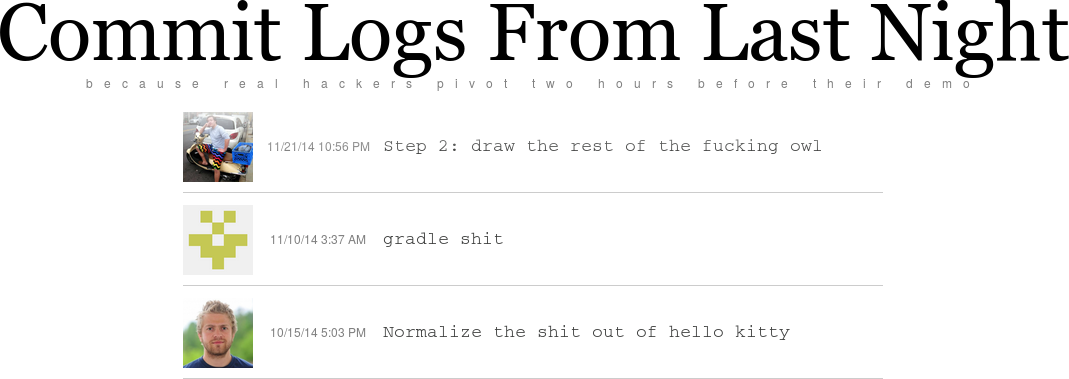
\includegraphics[width=\textwidth]{img/clfln}
    \begin{description}
        \fitem[Research Question:] Frustration Levels of Developers
        \fitem[Data Source:] Commit Messages on GitHub
        \fitem[Technologies Used:] \url{githubarchive.org}, List of Curse Words
    \end{description}
\end{frame}

\begin{frame}[fragile]
    \framecount{Related Work}
    \pause\vfill

    \Large\begin{Verbatim}[fontfamily=cmss]
Sentiment Analysis of Commit Comments in GitHub: An Empirical Studya
    \end{Verbatim}

    \normalsize
    \begin{description}
        \fitem[Research Questions:] Relation of Emotions to
        \begin{itemize}
            \fitem Programming Language
            \fitem Day of the Week or Time of Day
            \fitem Team's Geographical Distribution
            \fitem Project Approval
        \end{itemize}
        \fitem[Data Source:] 29 of top-starred GitHub projects
        \fitem[Technologies Used:] SentiStrength
    \end{description}
\end{frame}


%%%%%%%%%%%%%%%%%%%%%%%%%%%%%%%%%%%%%%%%%%%%%%%%%


\nextframe
\begin{frame}
    \vfill
    \begin{center}
        {\Huge Thank You All For Listening}\\
        $~$\\
        \url{https://github.com/hartenfels/Commit-Rater}
    \end{center}
\end{frame}

\end{document}
